\documentclass{article}
% To include code color syntaxing
\usepackage{minted}
% To include images
\usepackage{graphicx}
% To define margins
\usepackage[a4paper,left=2.5cm,right=2.5cm,top=2.5cm,bottom=2.5cm]{geometry}
% To comment multiple lines
\usepackage{comment}
% To use hyperlink
\usepackage{hyperref}
% To write formulas and equations
\usepackage{amsmath}
\usepackage{adjustbox}
% Setting all hyperlinks color to black, then setting only url colors to blue
\hypersetup{
  colorlinks,
  allcolors=.,
  urlcolor=blue,
}

\begin{document}

\begin{titlepage}
	\begin{center}
		\huge{\bfseries II.2315 – Project : Advanced algorithm and programming} \\
		\rule{16cm}{0.4pt} \\
		\huge{\bfseries Australia - Canberra} \\
		\vspace{3mm}
		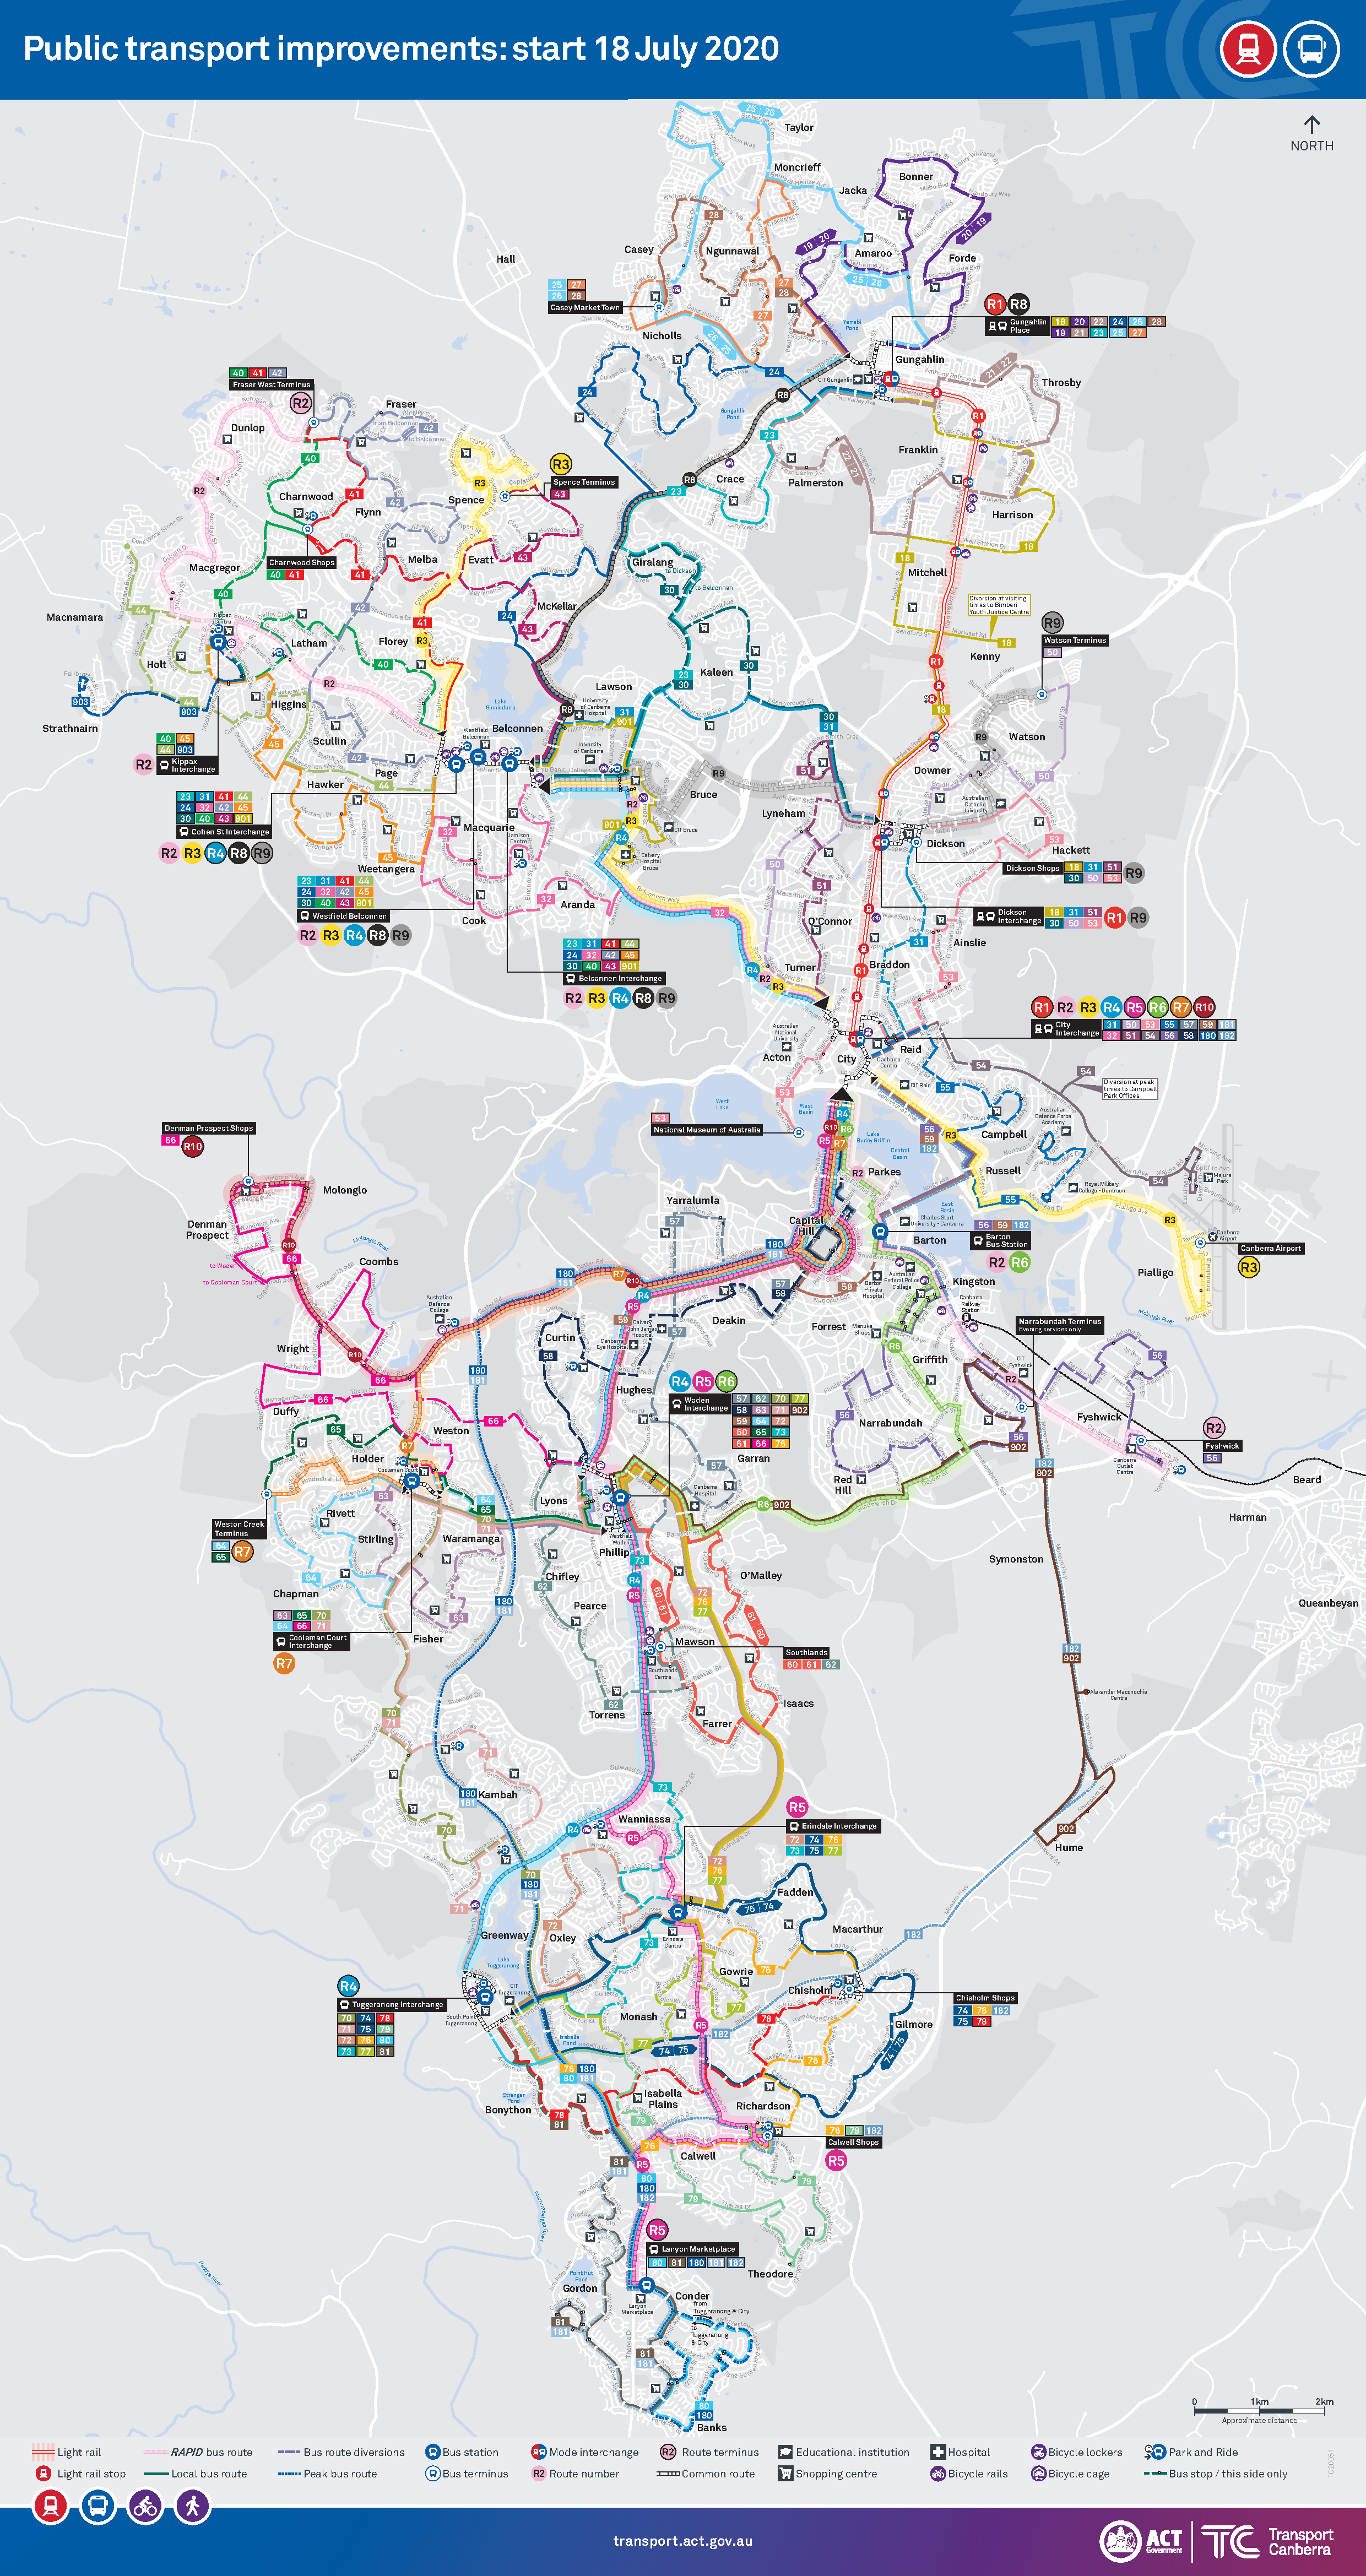
\includegraphics[scale=0.20]{assets/CanberraMap}
		\rule{16cm}{0.4pt} \\
		\vspace{5mm}
		
\includegraphics[scale=0.20]{assets/logoISEP} \\
		\textsc{\large Sarah HEOUAINE - David LAMY-VERDIN - Elia TSO}
		\medbreak
		\textsc{\large 2020 - 2021}
	\end{center}
\end{titlepage}

\renewcommand{\contentsname}{Table of contents}
\tableofcontents
\cleardoublepage

\section{Introduction}

\subsection{City of choice}

	We selected the city of Canberra, capital of Australia, for our project. This city has a total of 2433 stations and 2759 links.
	
\subsection{Goals of the project}

	This project had for first goal to create a graph representing the transport map of Canberra out of mere data. After this graph has been created, we could use it to reach other goals described in the below list:
	
\begin{itemize}
\item[-] Search algorithms \\
Implementation of the Bread-First Search Algorithm \\
Implementation of the Dijkstra Algorithm
\medbreak
\item[-] Applications of those algorithms \\
Searching for shortest paths \\
Splitting the map into clusters
\end{itemize}

	Through this project, optimization also had to be done as searching for shortest paths and splitting into clusters a graph as large as Canberra Transport Map was particularly demanding on resources and took a considerable amount of time.
	
\subsection{Collection of data : GTFS files}
	
	To build our graph, we used data retrieved from \href{https://www.transport.act.gov.au/contact-us/information-for-developers}{Australia Government official website}. This data come as multiple \textit{.txt} files. After studying them, it has been figured out that only \textit{stops.txt} and \textit{stop\_times.txt} were actually useful.
	
\begin{figure}[h]
\begin{center}
	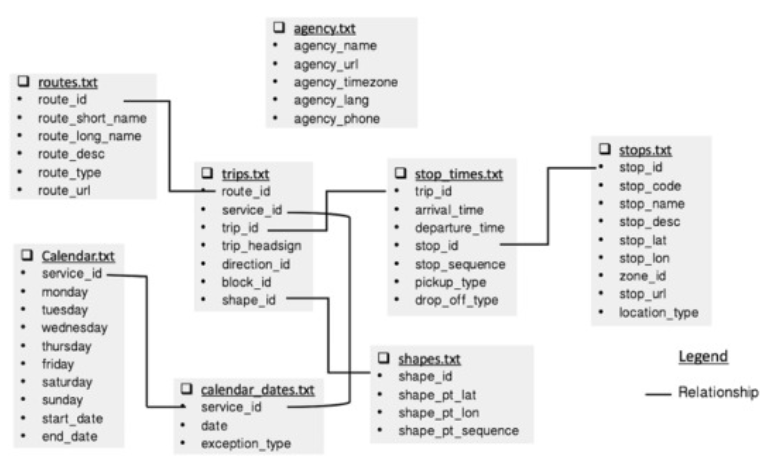
\includegraphics[scale=1]{assets/data}
\end{center} 
\caption{Data included in each \textit{.txt} file and relations between them}
\end{figure} 


	Using only those, we could create the stations which are represented in our graph as nodes and we could also link each of them and thus creating our edges.
	
\newpage
	
	The \textit{stops.txt} file provide us with \textit{stop\_id},  \textit{stop\_lat}, \textit{stop\_lon} which are all the information we needed to create our nodes while the \textit{stop\_times.txt} give us \textit{trip\_id} which allow us to create our edges. A trip informs about which stations are linked together and in which order as it defines a bus or subway line such as the R3 line of Canberra for example:
	
\begin{figure}[h]
\begin{center}
	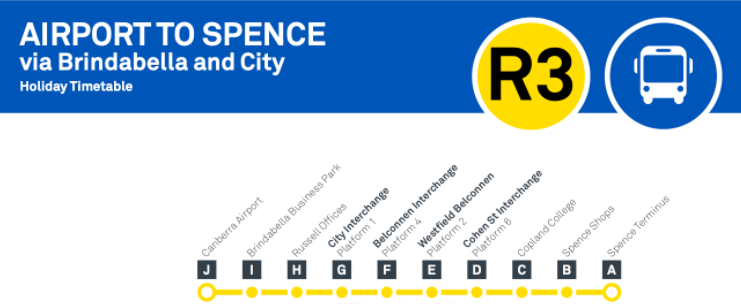
\includegraphics[scale=1]{assets/R3}
\end{center}
\caption{R3 bus line of Canberra}
\end{figure} 

\section{Creation of the graph}

\subsection{Graph}

\mintinline{java}{Graph.java} is the class used for building graphs.
The class contains the three following attributes:

\begin{itemize}
\item[-]\mint[breaklines, breaksymbolleft=]{java}{private Map<Integer, List<DirectedEdge>> map = new TreeMap<Integer,List<DirectedEdge>>()} This \mintinline{java}{Map} is used to store the adjacency lists of every node of our graphs. Each \mintinline{java}{Key} of the \mintinline{java}{Map} designates a node of our graph and the corresponding \mintinline{java}{Value} of the \mintinline{java}{Map} is its adjacency list. The choice to use a \mintinline{java}{Map} over a \mintinline{java}{List} is because unlike graphs where nodes labels are consecutive numbers, the stations of Canberra are not labeled consecutively. Therefore, using a \mintinline{java}{Map} makes it easier to look for an adjacency list of a specific station. This would not have been possible with a \mintinline{java}{List}. 
\item[-]\mintinline{java}{private boolean weighted} indicates if the graph is weighted or not.
\item[-]\mintinline{java}{private boolean directed} indicates if the graph is directed or not.
\end{itemize}

	Besides these attributes, \mintinline{java}{Graph.java} also has several methods whose most important ones are the following:

\begin{itemize}
\item[-]\mint[breaklines, breaksymbolleft=]{java}{private void convertTxt(File stopsFile, File stopTimesFile, boolean weighted, boolean directed)}
\item[-]\mint{java}{private void addNodesFromTxt(File stopsFile)}
\item[-]\mint{java}{private void addEdgesFromTxt(File stopTimesFile)}
\item[-]\mint{java}{private void addWeightsFromTxt(File stopsFile)}
\end{itemize}

\begingroup
\setlength{\rightskip}{0pt plus 1 fil}
The first method is used to initialize a graph by calling the other three methods and in the meantime setting the attributes \mintinline[breaklines, breakafter=_]{java}{private boolean weighted} and \mintinline{java}{private boolean directed}.
\endgroup

The other three methods are used to parse \textit{stops.txt} and \textit{stop\_times.txt}, retrieve the data and create the nodes and edges of our graph.

\subsection{Nodes}

For \textit{stops.txt}, each line was containing these informations in this order: stop\_id, stop\_name, stop\_lat, stop\_lon. In order to create our nodes, we had to use the stop\_id as labels for our nodes. To do so, the method \mintinline{java}{private void addNodesFromTxt(File stopsFile)} has been created.

\begin{figure}[h]
\begin{minted}[breaklines]{java}
private void addNodesFromTxt(File stopsFile) throws FileNotFoundException {

	Scanner myReader = new Scanner(stopsFile);
	myReader.nextLine(); // skip headers line
	int stop_id;
		
	while (myReader.hasNextLine()) {
			
		// split the line
		String line = myReader.nextLine();
		String[] arr = line.split(",");
		
		// add the id of the node
		stop_id = Integer.parseInt(arr[0]);
		if (this.map.containsKey(stop_id)) {
			System.out.println("Node in duplicate: " + stop_id);
		} else {
			List<DirectedEdge> list = new ArrayList<DirectedEdge>();
	this.map.put(stop_id, list);
		}
			
	}
}	
\end{minted}
\caption{\mintinline{java}{private void addNodesFromTxt(File stopsFile)}}
\end{figure}


The method takes the \textit{stops.txt} as input and reads every line as a \mintinline{java}{String} using \mintinline{java}{java.util.Scanner}. After splitting the \mintinline{java}{String} using a comma as separator, the method then retrieves the first element of the output array which corresponds to stop\_id and creates a new \mintinline{java}{Entry} to the \mintinline{java}{Graph Map} using the stop\_id as \mintinline{java}{Key} and an empty \mintinline{java}{List<DirectedEdge>} as \mintinline{java}{Value} only if the \mintinline{java}{Graph Map} does not already contain this \mintinline{java}{Key}

\subsection{Edges}

For \textit{stop\_times.txt}, the informations are disposed as below: trip\_id, arrival\_time, departure\_time, stop\_id, stop\_sequence, timepoint. As above, the method \mintinline{java}{private void addEdgesFromTxt(stopTimesFile)} takes \textit{stop\_times.txt} as input and split each line into an array using commas as separators.

The interesting data in {stop\_times.txt} is both trip\_id and stop\_id. If from a line to the other, the trip\_id is the same, we know that both stations of each line are part of the same bus or subway line and are therefore linked together by and edge.
As the method has to link each line to the previous one to check if the trip\_ id is the same and to create the edge between the two stop\_id, we store the data of the current iteration as well as of the previous iteration.

\newpage

\begin{figure}[H]
\begin{minted}[breaklines]{java}
[...]
if (directed){
	// if we are still in the same trip, then the 2 stations are connected
	if (trip_id.equals(trip_id0)) { 
		if (!this.map.containsKey(stop_id0)) {
			System.out.println("Node does not exist: " + stop_id0);
		} else {
			List<DirectedEdge> edgesList = this.map.get(stop_id0);
			boolean exists = false;
			for (int i = 0; i < edgesList.size(); i++) { // to avoid duplicates
				if (edgesList.get(i).to() == stop_id) {
					exists = true;
					break;
				}
			}
			if (!exists) {
				DirectedEdge newEdge = new DirectedEdge(stop_id0, stop_id, 1);
				edgesList.add(newEdge);
			}
		}
	}
} else if (!directed){
	if (trip_id.equals(trip_id0)) { 
		if (!this.map.containsKey(stop_id0)) {
			System.out.println("Node does not exist: " + stop_id0);
		} else if (!this.map.containsKey(stop_id)) {
			System.out.println("Node does not exist: " + stop_id);
		} else {	
			List<DirectedEdge> edgesList0 = this.map.get(stop_id0);
			List<DirectedEdge> edgesList = this.map.get(stop_id);
			boolean exists = false;
			for (int i = 0; i < edgesList0.size(); i++) { // to avoid duplicates
				if (edgesList0.get(i).to() == stop_id) {
					exists = true;
					break;
				}
			}
			if (!exists) {
				DirectedEdge newEdge0 = new DirectedEdge(stop_id0, stop_id, 1);
				DirectedEdge newEdge = new DirectedEdge(stop_id, stop_id0, 1);
				edgesList.add(newEdge);
				edgesList0.add(newEdge0);
			}
		}
	}
}
[...]
\end{minted}
\vspace*{-10mm}\caption{\mintinline{java}{private void addEdgesFromTxt(File stopTimesFile)}}
\end{figure}

The method then checks if the nodes are actually existing and if they do, add the edge to the right adjacency list:

\begin{itemize}
\itemsep0em 
\item[-] only to the source node adjacency list if the graph is directed
\item[-] to both the source and destinations nodes adjacency lists if the graph is not directed
\end{itemize}

\newpage

\subsection{Weights}

\begin{figure}[h]
\begin{minted}[breaklines]{java}
[...]
for (Map.Entry<Integer,List<DirectedEdge>> entry : this.map.entrySet()) {
	for (DirectedEdge edge : entry.getValue()) {
		source = edge.from();
		destination = edge.to();
		sourceLat = mapCoord.get(source).getLatitude();
		sourceLong = mapCoord.get(source).getLongitude();
		destinationLat = mapCoord.get(destination).getLatitude();
		destinationLong = mapCoord.get(destination).getLongitude();
		distance = Math.sqrt(Math.pow((destinationLat-sourceLat),2) + Math.pow((destinationLong-sourceLong),2));
		edge.setWeight(distance);
	}
}
[...]
\end{minted}
\caption{\mintinline{java}{private void addWeightsFromTxt(File stopsFile)}}
\end{figure}

The method \mintinline{java}{private void addWeightsFromTxt(File stopsFile)} is used only if the graph is weighted. It takes \textit{stops.txt} as input and extracts both stop\_lat and stop\_lon for each station to store it into a \mintinline{java}{Map} of \mintinline{java}{Coordinates} which is a \mintinline{java}{Class} that simply has stop\_lat and stop\_lon as attributes. Once the \mintinline{java}{Map} of \mintinline{java}{Coordinates} created, the method calculates the euclidean distance between starting node and destination node for every edge of the graph and set it as weights.

\begin{figure}[h]
\begin{gather*}
  d(a,b) = \sqrt{(a_{lon} - b_{lon})^2 + (a_{lat} - b_{lat})^2}, \\
  \text{where~$a$ is the starting node,~$b$ is the destination node}
\end{gather*}
\caption{Euclidean distance formula in two dimensions}
\end{figure}

Here is an example of what this method would give for the R3 bus line of Canberra:

\begin{center}
\begin{figure}[h]
\begin{adjustbox}{max width=\textwidth}
\begin{tabular}{ |c|c|c|c|c|c|c| } 
 \hline
 stop\_id: source & stop\_lat: source & stop\_lon: source & stop\_id: destination & stop\_lat: destination & stop\_lon: destination & distance \\ 
 \hline
 3353 & -35.307607 & 149.189463 & 3467 & -35.316348 & 149.190329 & 0.008783793998 \\ 
 \hline
 3467 & -35.316348 & 149.190329 & 3011 & -35.297298 & 149.150267 & 0.04436063958 \\
 \hline
 3011 & -35.297298 & 14.150267 & 3419 & -35.278322 & 149.12815 & 0.02914189879 \\
 \hline
 3419 & -35.278322 & 149.12815 & 5514 & -35.240007 & 149.067995 & 0.07132084723 \\
 \hline
 5514 & -35.240007 & 149.067995 & 5502 & -35.23861 & 149.063546 & 0.004663175956 \\
 \hline
 5502 & -35.23861 & 149.063546 & 940 & -35.24 & 149.060282 & 0.003547646544 \\
 \hline
 940 & -35.24 & 149.060282 & 4072 & -35.21243 & 149.0607 & 0.02757316855 \\
 \hline
 4072 & -35.21243 & 149.0607 & 4091 & -35.194784 & 149.060626 & 0.01764615516 \\
 \hline
 4091 & -35.194784 & 149.060626 & 4807 & -35.200702 & 149.068587 & 0.009919689763 \\
 \hline
 4807 & -35.200702 & 149.068587 & X & X & X & X \\ 
 \hline
\end{tabular}
\end{adjustbox}
\caption{Table of coordinates and distances for edges of the R3 bus line of Canberra}
\end{figure}
\end{center}

\section{Breadth-First Search}

The Breadth-First Search algorithm has been implemented in the \mintinline{java}{BFSSP.java}. Methods of this class have all been made \mintinline{java}{static} as it is not necessary to store any data from one breadth-first search to the other. An user would likely use a breadth-first search on the graph of his choice and it makes more sense to just create a graph instead of having to create both a graph and a \mintinline{java}{BFS} instance. The method \mintinline{java}{public static List<Integer> bfs(Graph G, int startingNode)} takes a graph and a starting node as parameters and starts a breadth-first search.

While doing a breadth-first search, we need to store for each node three values:
\begin{itemize}
\item[-]\mintinline{java}{private boolean marked} to know if the node has been reached at some point during the breadth-first search
\item[-]\mintinline{java}{private int previous} to know which node preceded the node during the breadth-first search
\item[-]\mintinline{java}{private int distance} to know the distance separating the node to the starting node of the breadth-first search
\end{itemize}

Just as for \mintinline{java}{Map} of \mintinline{java}{Graph.java}, it is more intuitive to use a \mintinline{java}{Map} to store all of these values. One approach could be to use three different \mintinline{java}{Map}, however, to use less memory and make the code more efficient we decided to use a single \mintinline{java}{Map} whose entries would store a tuple of three elements. This tuple contains a \mintinline{java}{boolean}, and two \mintinline{java}{int} and results in the creation of the \mintinline{java}{class} \mintinline{java}{MPD.java}.

\begin{minted}[breaklines]{java}
public static List<Integer> bfs(Graph G, int startingNode) {
	List<Integer> path = new ArrayList<Integer>();
	List<Integer> toVisitNodes = new ArrayList<Integer>();
	for (Integer key : G.getMap().keySet()) {
		mapMPD.put(key, new MPD(false, -1, 0.0));
	}
	toVisitNodes.add(startingNode);
	mapMPD.put(startingNode, new MPD(false, -1, 0.0));
	
	if (G.isWeighted()) {
		
		System.out.println("Please consider using Dijkstra Algorithm on weighted graph if you would like to find shortest paths.");
		
	}
		
		while (!toVisitNodes.isEmpty()) {

			int currentNode = toVisitNodes.remove(0);
			mapMPD.get(currentNode).marked = true;
			path.add(currentNode);
			
			for (DirectedEdge edge : G.getMap().get(currentNode)) {
				if (!toVisitNodes.contains(edge.to()) && !mapMPD.get(edge.to()).marked) {
					toVisitNodes.add(edge.to());
					mapMPD.get(edge.to()).previous = currentNode;
					mapMPD.get(edge.to()).distance = mapMPD.get(currentNode).distance+1;					
				}
			}
		}
	//}
	return path;
}	
\end{minted}

When doing the breadth-first search, the first thing to do is to check whether or not the graph given in parameter is weighted or not.  If it is weighted, the method warns the user that the breadth-first search cannot be used on weighted graph to look for shortest paths. However, it stills runs the breadth-first search, as even though it cannot be used to find shortest paths, it could still be used to discover connected nodes on a weighted graph.

\newpage

The breadth-first search works as follows:
\begin{itemize}
\item[$\bullet$] Adds starting node given in parameter  to \mintinline{java}{toVisitNodes} which is the list of nodes the method is planning to visit
\item[$\bullet$] Sets the first element of \mintinline{java}{toVisitNodes} as the current node and removes it from list ; sets its \mintinline{java}{MPD.marked} attribute to \mintinline{java}{true}
\item[$\bullet$] For every neighbor of the current node, if the neighbor is not marked yet and if the neighbor is not contained in \mintinline{java}{toVisitNodes}
\item[$\bullet$] Loops until \mintinline{java}{toVisitNodes} is empty, meaning there is not any remaining connected node that has yet to be visited
\end{itemize}

\subsection{Shortest paths}

Assuming a breadth-first search has already been launched for the starting node of the shortest path the user is looking for. The shortest path can then first be printed.

Before printing a path, it is necessary to make sure this path actually exists. In order to do so, the method \mintinline{java}{public static boolean hasPathTo(int destination)} has been implemented. It simply returns a boolean indicating if a path exists or not. It can be done easily as the \mintinline{java}{marked} attribute of \mintinline{java}{MPD} solely serves this purpose and just returning its value does the trick.

\mintinline{java}{public static printShortestPath(int startingNode, int destinationNode)} first checks if the path exists using \mintinline{java}{hasPathTo()}. If it does not, the code warns the user by printing a message. Another check done by the method is the egality of \mintinline{java}{startingNode} and \mintinline{java}{destinationNode}. If these nodes are the same, there is no need to continue.

Once these checks done, if a path exists and the starting node is distinct from the destination node, the starts loooking for the shortest path. It does so by browsing \mintinline{java}{MPD.previous} attribute starting from the destination node and going all the way back to the starting node. As the path is discovered from destination to start, the code builds the path backwards.

\section{Dijkstra Algorithm}


\end{document}
